\documentclass[xcolor=table]{beamer}

\mode<presentation> {
\usetheme{Madrid}
}

\usepackage{graphicx}
\usepackage[utf8]{inputenc} 
\usepackage[french]{babel}

\usepackage{multirow}
\usepackage[table]{xcolor}

\title[M1SSI]{Authentification \`{a} base d'OTP}

\institute[Universit\'{e} de Rouen] {
Universit\'{e} de Rouen \\
\medskip
}
\date{\today}

\begin{document}

\begin{frame}
\titlepage
\end{frame}

\begin{frame}
\frametitle{Table des mati\`{e}res}
\tableofcontents
\end{frame}

%------------------------------------------------
\section{Pr\'{e}sentation}
%------------------------------------------------

\subsection{Qu'est ce qu'un OTP}

\begin{frame}
\frametitle{Description OTP}
\begin{block}{Définition}
    Un OTP est un mot de passe jetable, c'est à dire qu'il satisfait les deux 
  critères suivants:
  \begin{itemize}
    \item Il n'est pas prédictible
    \item Il n'est valide que pour une unique session.
  \end{itemize}
\end{block}

\begin{block}{Utilité}
  \begin{itemize}
    \item Permettre une authentification forte.
    \item Éviter les attaques par rejeu.
  \end{itemize}
\end{block}
\end{frame}

\subsection{Demande du client}

\begin{frame}
\frametitle{Le livrable}
\begin{block}{Etat de l'art} 
Un état de l'art comprenant au moins trois protocoles OTP étudiés.
\begin{description}
 \item[OTP] Protocole de base.
 \item[HOTP] Protocole utilisant la fonction HMAC et un compteur de 
  synchronisation.
 \item[TOTP] Protocole reprenant HOTP avec le temps comme compteur.
 \item[EAP-POTP] Architecture pour s'authentifer sur \verb?IEEE 802.1x?. 
 \item[OTPW] Protocole basé sur l'état de la machine et la fonction de hashage RIPEMD-160.
\end{description}
\end{block}
\end{frame}

\begin{frame}
\frametitle{Le livrable}
\begin{block}{Application}
    L'application se fera sur les protocole qui auront été retenu après l'étude de 
  l'état de l'art et comportera pour chaque protocole:
  \begin{itemize}
    \item Un serveur d'authentification
    \item Un client d'authentification
    \item Un token\footnote[1]{Programme permettant à l'utilisateur d'obtenir un 
      OTP pour s'authentifer.}\footnote[2]{Tout les protocoles ne 
      nécessitent pas de tokens.} android
    \item Un token Linux
  \end{itemize}
\end{block}

\end{frame}


%------------------------------------------------
\section{Organisation du travail}
%------------------------------------------------

\subsection{Méthodologie}
\begin{frame}
\frametitle{Méthodologie}
\begin{center}
\Huge eXtreme Programming
\normalsize
\begin{block}{Les grands principes}
\begin{itemize}
 \item Test Driven Developpement
 \item Intégration continue et Refactoring
 \item Appropriation collective du code
 \item Programmation en binôme
\end{itemize}
\end{block}
\end{center}

\end{frame}

\subsection{Organisation des taches}
\begin{frame}
\frametitle{Formation des equipes de travail}
\begin{block}{Équipe lors de l'état de l'art}
  \begin{itemize}
    \item POTP
    \begin{itemize}
      \item Tayewo-John-Yves \bsc{ADEGOLOYE}
      \item Claire \bsc{HARDOUIN}
    \end{itemize}
    \item HOTP - TOTP
    \begin{itemize}
      \item Gaëtan \bsc{FERRY}
      \item Maxime \bsc{MICHOTTE}
      \item Benjamin \bsc{ZIGH}
    \end{itemize}
    \item OTPW - OTP
    \begin{itemize}
      \item Damien \bsc{PICARD}
      \item Adrien \bsc{SMONDACK}
    \end{itemize}
  \end{itemize}
\end{block}
\end{frame}



%------------------------------------------------
\section{Aspect technique}
%------------------------------------------------

\subsection{Langages}
\begin{frame}
\frametitle{Technique}
\begin{block}{Technologies utilisés}
\begin{itemize}
  \item Pour le serveur et le token Linux le C est de rigueur.
  \item Pour le token android nous comptons utiliser Java. 
\end{itemize}
\end{block}
\end{frame}

\subsection{Architecture logicielle}
\begin{frame}
\frametitle{Technique}
\begin{figure}
 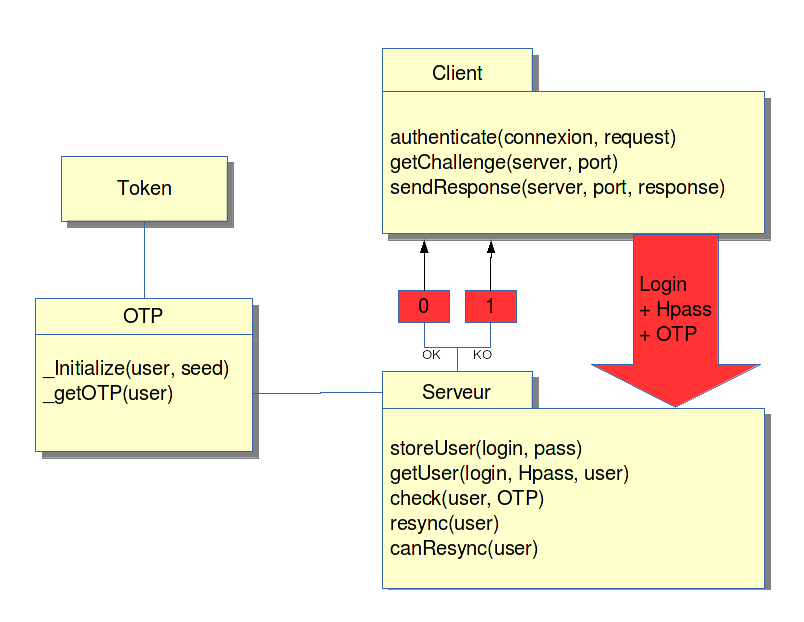
\includegraphics[scale=0.3]{img/architecture.png} 
 \caption{Schéma de l'architecture logicielle}
\end{figure}

\end{frame}


%------------------------------------------------
\section{Tests et vérifications}
%------------------------------------------------

\begin{frame}
  \frametitle{Tests et vérifications}
  \begin{itemize}
   \item Procédures de tests écrites au début du développement de chaque composante. (test driven developement)
   \item Tests exécutés par les équipes de développement tout au long du processus de création.
   \item  Lorsque des anomalies sont détectées lors des tests, la procédure est la suivante:
    \begin{itemize}
     \item Création d'une note / mémo précisant l'anomalie rencontrée.
     \item Ajout d'une entrée au journal de test précisant la date du test.
     \item Diffusion de la note à l'équipe de développement pour correction.
    \end{itemize}
  \end{itemize}
\end{frame}


%------------------------------------------------
\section{Plan de développement}
%------------------------------------------------
\begin{frame}
\frametitle{Planning Poker}
  \begin{figure}
    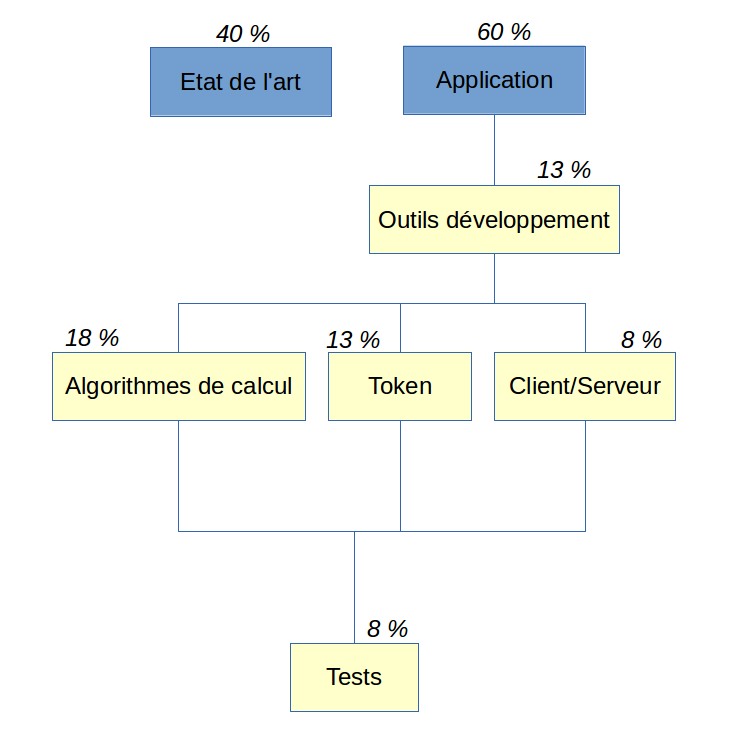
\includegraphics[scale=0.3]{img/planningpoker.png}
    \caption{Planning poker}
  \end{figure}
\end{frame}

\begin{frame}
\frametitle{Schéma Macroscopique du Projet}
\begin{figure}[h]
  \centering
  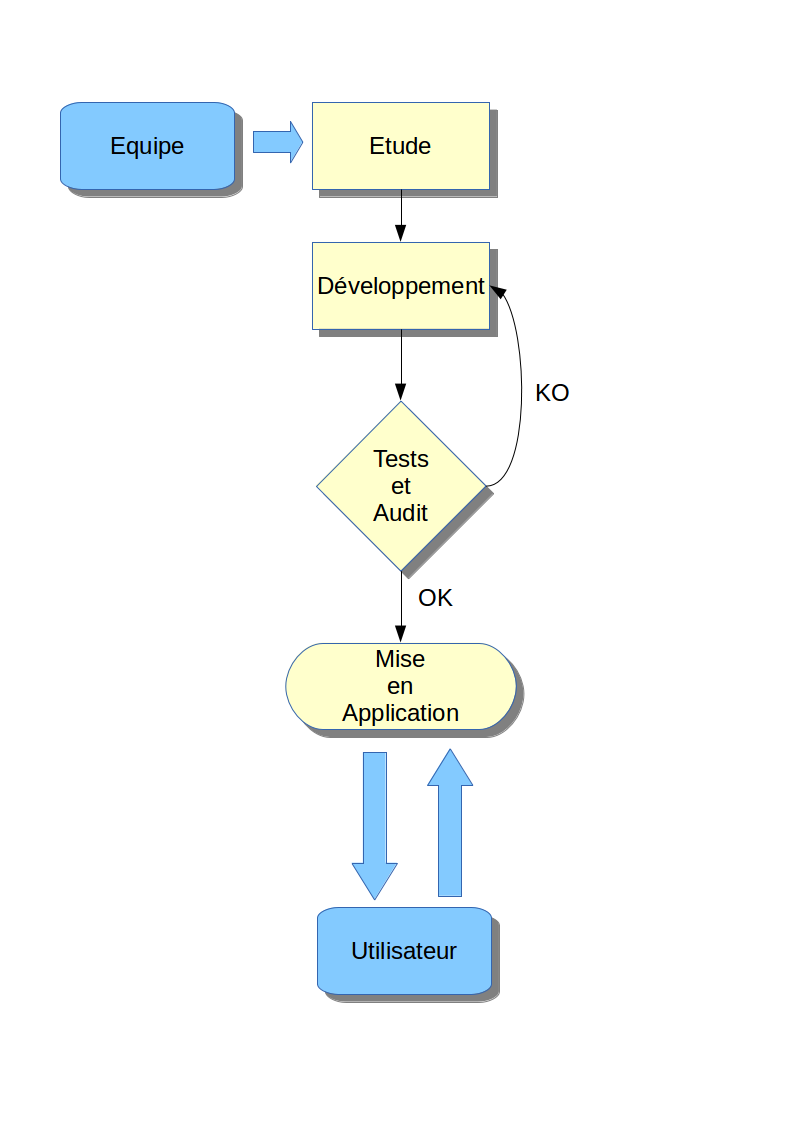
\includegraphics[scale=0.2]{../graphics/diagramme1.png}
  \caption{Schéma Macroscopique du Projet}
  \setlength{\parindent}{1cm}
\end{figure}
\end{frame}

\begin{frame}
\frametitle{Diagramme de Gantt}
  \begin{figure}
    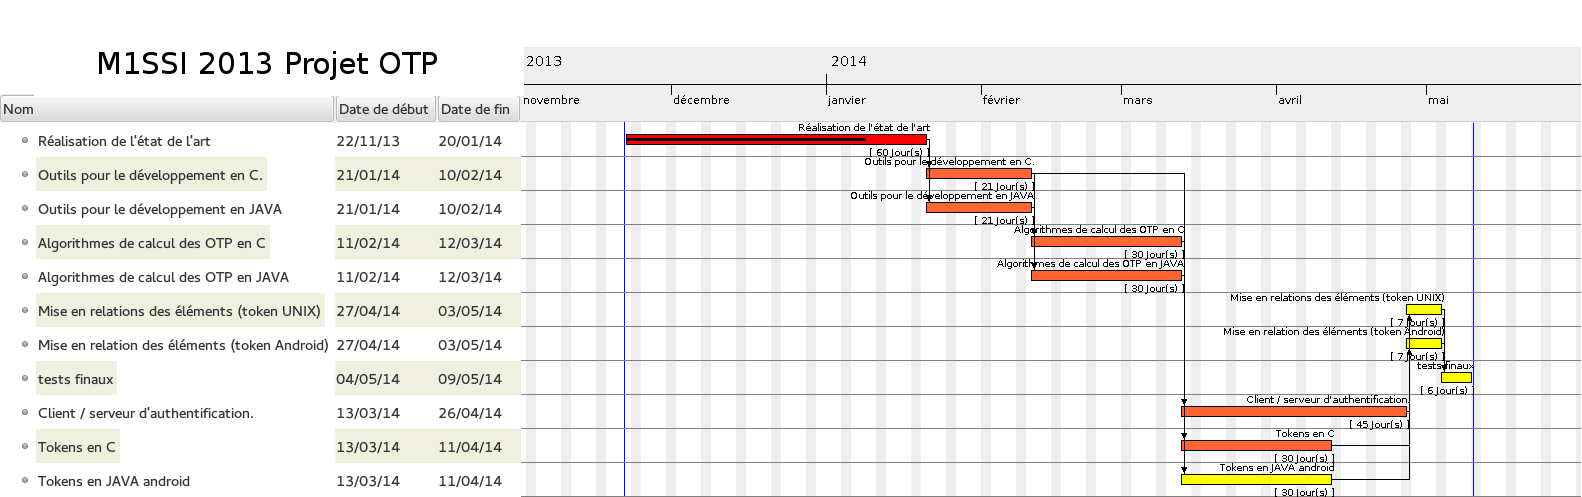
\includegraphics[scale=0.22]{img/gantt.png}
    \caption{Planning des étapes du projet}
  \end{figure}
\end{frame}

%------------------------------------------------
\section{Gestion des risques}
%------------------------------------------------

\begin{frame}[fragile]
\frametitle{Gestions des risques}
  \begin{center}
  \begin{tabular}{| p{5cm} | p{2cm} |p{2cm} |}
  \hline
  \rowcolor{lightgray}Libelle & Impact & Probabilité\\ \hline
  Retard pour une partie de l'équipe (compréhension et/ou compétences) & \textcolor{orange}{Préoccupant} & \textcolor{red}{forte}\\ \hline
  Appréhension des nouvelles technologies plus longue que prévu & \textcolor{orange}{Préoccupant} & \textcolor{red}{forte}\\ \hline
  Faille de sécurité découverte après test. & \textcolor{red}{Important} & \textcolor{orange}{Moyenne}\\ \hline
  Phase de développement plus longue que prévu.& \textcolor{red}{Important} & \textcolor{red}{forte}\\ \hline
  Impondérables (surcharge de travail).& \textcolor{red}{Important} & \textcolor{red}{forte}\\ \hline
  \end{tabular}
  \end{center}
\end{frame}

%------------------------------------------------
\section{Conclusion}
%------------------------------------------------

\subsection{En Conclusion}

\begin{frame}
\frametitle{Conclusion}
  \begin{itemize}
   \item Le projet est réalisable (ref Diagramme de Gantt).
  \end{itemize}
\end{frame}
%------------------------------------------------
\end{document}